\documentclass[tikz,border=5]{standalone}
\usetikzlibrary{circuits.ee.IEC,calc}
\begin{document}
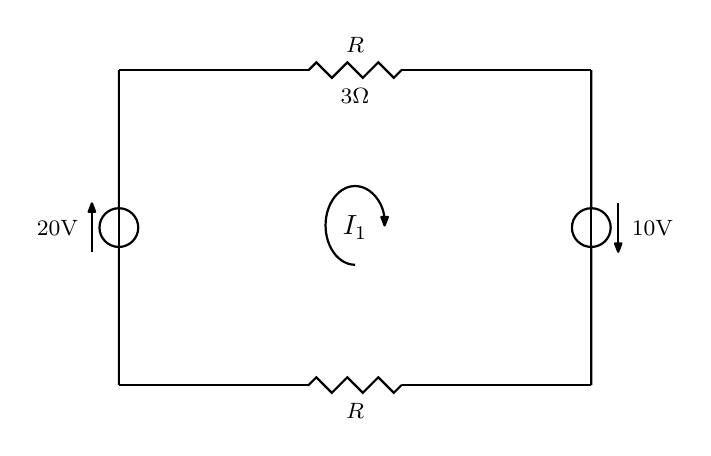
\begin{tikzpicture}[circuit ee IEC, x=3cm, y=4cm, thick, 
  every info/.style={font=\footnotesize},
  set resistor graphic=var resistor IEC graphic,
  set diode graphic=var diode IEC graphic,
  set make contact graphic= var make contact IEC graphic,
  circuit declare annotation={circular annotation}{0}
    { (270:3/16) edge [to path={ arc (270:0:1/8) } ] () }]

\draw (0,0)  to [voltage source={direction info={volt=20}}] ++(0,1);
\draw (0,1)  to [resistor={info={$R$},ohm'=3}]  (2,1);
\draw (2,1)  to [voltage source ={direction info={volt=10}}] (2,0);
\draw (2,0)  to [resistor={info=$R$}] (0,0);
\node at (1,1/2) [circular annotation] {$I_1$};
\end{tikzpicture}
\end{document}
